\documentclass[a4paper]{article}

\usepackage[utf8]{inputenc}
\usepackage[spanish]{babel}
\usepackage[margin=2cm, top=2cm, includefoot]{geometry}%--para definir espacio de márgenes
\usepackage{graphicx}%--para insertar imágenes
\usepackage{fancyhdr}%--para el estilo con barra arriba de las páginas
\usepackage[table,xcdraw]{xcolor}%--para la detección de colores
\usepackage[hidelinks]{hyperref}%--para hipervínculos
\usepackage{parskip}%--para evitar tabulación de inicio de párrafo
\usepackage{booktabs}%--
\usepackage{tabularx}

%definiendo color
\definecolor{rojoOscuro}{HTML}{A20303}
%---definiendo estilo del informe
\setlength{\headheight}{47pt}
\pagestyle{fancy}
\fancyhf{}
\lhead{\hspace{0.1cm} 
\includegraphics[height=1.55cm]{imagenes/CiberSecFIIS.png}}\rhead{
\includegraphics[height=1.5cm]{imagenes/uni_logo.png} \hspace{0.1cm}}

%---Cambios
\renewcommand{\headrulewidth}{3pt}%--grosor de la linea superior
\renewcommand{\headrule}{\hbox to\headwidth{\color{rojoOscuro}\leaders\hrule height \headrulewidth\hfill}}%--definir la linea base superior
\renewcommand{\arraystretch}{2.5}%--espaciado de las tablas
%---Inicio de informe
\begin{document}
    \begin{titlepage}
    \centering
        {\large \textbf{UNIVERSIDAD NACIONAL DE INGENIERÍA}} \par \vspace{0.3cm}
        {\large \textbf{FACULTAD DE INGENIERÍA INDUSTRIAL Y DE SISTEMAS}} \par \vspace{1.125cm}
        
\includegraphics[width=0.7\textwidth]{imagenes/CiberSecFIIS.png} \par \vspace{1.125cm}
        {\LARGE \textbf{Segunda Evaluación de Penetración de Seguridad}}\par \vspace{1cm}
        {\Large \textbf{Elaborado por:}} \par \vspace{1cm}
        {\large \textbf{Elian Paucar}} \par \vspace{0.8cm}
        {\large \textbf{Rodrigo Rojas}} \par \vspace{0.8cm}
        {\large \textbf{Sandro Castillo}} \par \vspace{2.75cm}
        \vfill
        {\textbf{Lima, 2021}}
\end{titlepage}
%-----------------------------------------------------------
    \clearpage
        \tableofcontents
    \clearpage
%------------------------------------------------------------
    \listoffigures
    \clearpage
%------------------------------------------------
    %----Para el inicio de numeración a partir de aquí---
    \cfoot{\thepage}
    \setcounter{page}{1}
 %--------Resumen ejecutivo------------
 \addcontentsline{toc}{section}{Resumen Ejecutivo} %--Para que sección sin numeración aparezca en el índice
    \begin{center}
        \section*{Resumen Ejecutivo}
    \end{center}
\vspace{0.1cm}
\begin{large}
El presente informe contiene todas las acciones realizadas por miembros del grupo CibersecFIIS para realizar una evaluación de seguridad y pruebas de penetración a cuatro computadoras pertenecientes a la plataforma Hack The Box.
\\
El propósito de este informe es evaluar y mejorar los conocimientos en ciberseguridad del equipo auditor haciendo uso de la plataforma Hack The Box.
\\
El actual informe detalla el alcance de las pruebas realizadas y los hallazgos importantes junto con las recomendaciones para mitigar vulnerabilidades. A continuación, se proporciona un resumen de los hallazgos clave descubiertos durante la evaluación.
\\
La cantidad de vulnerabilidades encontradas por máquina se resume en el siguiente gráfico.
\end{large}
\begin{figure}[h]
    \centering
    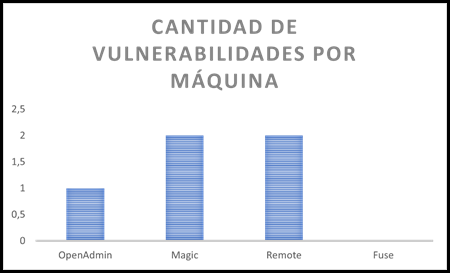
\includegraphics[width=0.7\textwidth]{imagenes/vuln_x_maq.png}
    \caption{Cantidad de vulnerabilidades por máquina}
\end{figure}

\large{El total de vulnerabilidades encontradas según su tipología se distribuyen de la siguiente forma:}
\\
\begin{figure}[h]
    \centering
    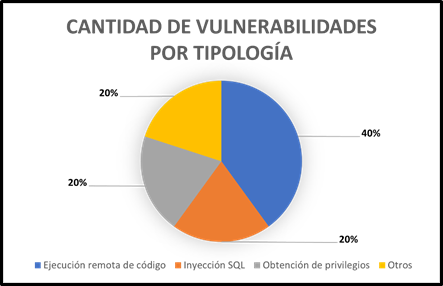
\includegraphics[width=0.7\textwidth]{imagenes/vuln_x_tipo.png}
    \caption{Cantidad de vulnerabilidades por tipología}
\end{figure}
\\
\large{De las 5 vulnerabilidades, solo 2 tienen identificador CVE asociado.}
\\
\\
\large{La cantidad de debilidades encontradas por máquina durante las pruebas de penetración se resume de la siguiente forma.}
\begin{figure}[h]
    \centering
    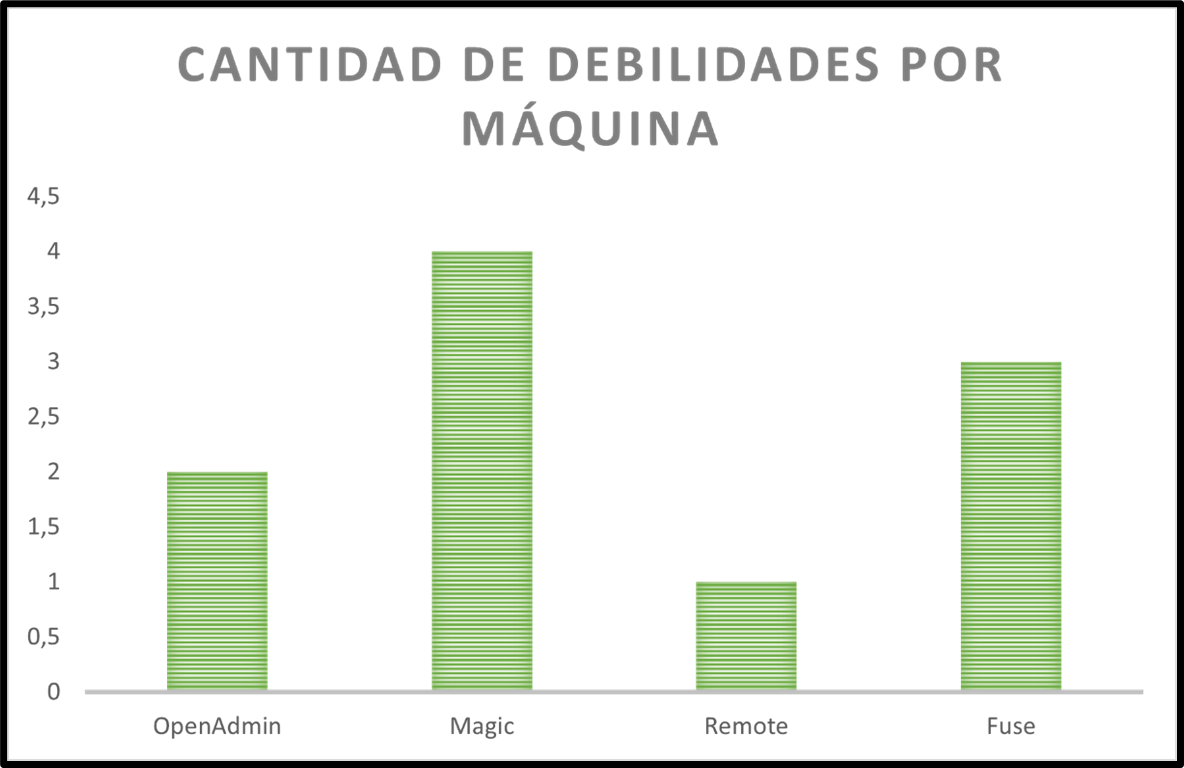
\includegraphics[width=0.7\textwidth]{imagenes/deb_x_maq.png}
    \caption{Cantidad de debilidades por máquina}
\end{figure}
\\
\large{La cantidad de máquinas relacionadas a un tipo de debilidad se distribuyen en el siguiente gráfico.}
\\
\begin{figure}[h]
    \centering
    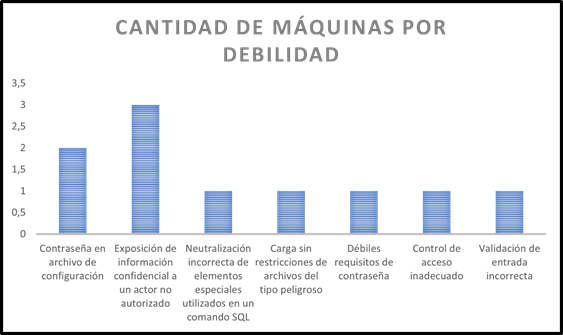
\includegraphics[width=0.7\textwidth]{imagenes/maq_x_deb.png}
    \caption{Cantidad de máquinas por debilidad}
\end{figure}
\\
\large{Según la cantidad de vulnerabilidades y debilidades en cada máquina, se puede observar que la máquina “Magic” es la más insegura con 2 vulnerabilidades y 4 debilidades.}

%-------------------------------------------------
\clearpage
\section{Objetivo}
\large{El objetivo de la presente evaluación de penetración de seguridad es encontrar vulnerabilidades y hacer una evaluación de criticidad de estas con el fin de que el negocio no se vea afectado por algún ataque malicioso que pueda afectar la calidad de sus servicios y su imagen.}
\section{Alcance}
\large{El alcance de esta evaluación se limita a las pruebas en los computadores de la plataforma Hack The Box con las siguientes direcciones IP:}
\par
\begin{table}[h]
    \centering
    \begin{tabular}{|c|c|c|c|c|} \hline
        Identificador & Nombre de host & Dirección IP & Sistema Operativo & Dificultad \\ \hline
        HTB01 & OpenAdmin & 10.10.10.171 & Linux & Fácil \\ \hline
        HTB02 & Magic & 10.10.10.185 & Linux & Medio \\ \hline
        HTB03 & Remote & 10.10.10.180 & Windows & Fácil \\ \hline
        HTB04 & Fuse & 10.10.10.193 & Windows & Medio \\ \hline
    \end{tabular}
    \caption{Datos sobre las máquinas}
\end{table}

\section{Detalle de Hallazgos}
\large{Los hallazgos encontrados en la evaluación de penetración de seguridad fueron los siguientes:}
\par
\vspace{0.1cm}
Se encontraron 5 vulnerabilidades, pertenecientes a 3 de 4 máquinas.
\par
\begin{table}[h]
    \centering
    \begin{tabular}{|c|c|c|c|c|c|c|c|} \hline
        \footnotesize{Identificador} & \footnotesize{CVE} & \footnotesize{Tipo de vulnerabilidad} & \footnotesize{CVSSv2} & \footnotesize{OpenAdmin} & \footnotesize{Magic} & \footnotesize{Remote} & \footnotesize{Fuse} \\ \hline
        \footnotesize{VU01} & - & \footnotesize{Ejecución Remota de Código} & - & \Large{\begin{math}\bullet\end{math}} &  &  &  \\ \hline
        \footnotesize{VU02} & - & \footnotesize{Inyección SQL} & - &  & \Large{\begin{math}\bullet\end{math}} &  &  \\ \hline
        \footnotesize{VU03} & \footnotesize{CVE-2017-6516} & \footnotesize{Obtención de privilegios} & \footnotesize{7.2} &  & \Large{\begin{math}\bullet\end{math}} &  &  \\ \hline
        \footnotesize{VU04} & - & \footnotesize{Ejecución Remota de Código} & - &  &  & \Large{\begin{math}\bullet\end{math}} &  \\ \hline
        \footnotesize{VU05} & \footnotesize{CVE-2019-1322} & \footnotesize{Otros} & \footnotesize{4.6} &  &  & \Large{\begin{math}\bullet\end{math}} &  \\ \hline
    \end{tabular}
    \caption{Vulnerabilidades encontradas}
\end{table}

\end{document}